\documentclass[a4paper,12pt]{article} %style de document
\usepackage[utf8]{inputenc} %encodage des caractères
\usepackage[french]{babel} %paquet de langue français
\usepackage[T1]{fontenc} %encodage de la police
\usepackage[top=2cm,bottom=2cm,left=2cm,right=2cm]{geometry} %marges
\usepackage{hyperref}
\usepackage{libertine}
\usepackage{xcolor,graphicx}
\newcommand{\HRule}{\rule{\linewidth}{0.5mm}}
\renewcommand{\baselinestretch}{1.5}
\addcontentsline{toc}{section}{\protect\numberline{}Introduction}
\usepackage[linesnumbered,ruled,french,onelanguage]{algorithm2e}


\begin{document}
\begin{titlepage}


\includegraphics[width = 20mm]{logo.png} \hfill
\begin{minipage}{0.4\textwidth}
\begin{flushright} \large
\today
\end{flushright}
\end{minipage}
\textsc{}\\[4cm]
\begin{center}

\HRule \\[2cm]

\textsc{\Large Rapport sur le Sokoban}\\[1.5cm]
\HRule \\[2cm]
\vspace{6cm}
\end{center}
 \begin{minipage}{0.4\textwidth}
      \begin{flushleft} \large
        Licence 2 Informatique
      \end{flushleft}
    \end{minipage}
    \begin{minipage}{0.6\textwidth}
      \begin{flushright} \large
       Pierre-Louis Klaeyle\\
       Laurine Mialon\\
       Max Jarrosay\\
       Gareth Lafay\\
      \end{flushright}
    \end{minipage}
\end{titlepage}
\tableofcontents
\newpage
\section*{Introduction}

Pour le second Semestre de L2 informatique, nous devions réaliser un projet en programmation orientée objet en groupe de 4 personnes cela dans le but de nous améliorer dans un nouveau langage de programmation : le Java.

Il nous a été présenté plusieurs projets, de notre coté nous nous sommes penchés sur le cas du Sokoban dont l’énoncé était :

«Sokoban est un jeu vidéo de puzzle dans lequel le joueur contrôle un personnage dans un entrepôt constitué de cases. Il doit alors ranger des caisses sur des cases cibles sachant que le personnage ne peut se déplacer que dans les quatre directions et pousser une seule caisse à la fois.Comme le personnage ne peut pas tirer de caisse, il est possible de se retrouver bloqué après un mouvement mal choisi. Ce projet a pour objectif de réaliser un jeu de Sokoban en permettant à un utilisateur de jouer en parallèle d'une intelligence artificielle et de comparer ses performances. Il s'agit de réaliser un jeu jouable pour un humain avec importation de niveaux. Pour cela, des formats de données (comme .xsb, .sok ou .stb) dédiés peuvent être utilisés. »

Nous avons donc composé notre travail en 3 parties :
\begin{itemize}
\item La réalisation du modèle d’un Sokoban.
\item Création d’une interface graphique avec Swing et Awt.
\item L’implémentation d’une intelligence artificielle.
\end{itemize}
\newpage
\section{Objectifs du projet}

\subsection{Présentation du Sokoban}
Le Sokoban est un jeu de puzzle créé en 1982 par Hiroyuki Imabayashi. A la base ce jeu se parcourait en solo à travers une cinquantaine de niveaux à la difficulté croissante.
Comme expliqué dans l’introduction le but du jeu est de pousser des caisses sur des cases cibles sans les coincer contre des murs.
Le jeu utilise des fichiers au format « .xsb » afin de stocker les différents niveaux. Ce format est le plus couramment utilisé a l’instar des format « .sok » et « .stb ». A l’intérieur de ces fichiers se trouve différents caractères qui représente les divers éléments présents sur la grille du Sokoban (voir le tableau ci-dessous).
\begin{table}[h]
\begin{center}
\begin{tabular}{|c|c|}
\hline
Caractère &
Signification \\
\hline
. &
Case cible\\
\hline
\$ &
Caisse \\
\hline
\# &
Mur \\
\hline
@ &
Personnage \\
\hline
* & 
Caisse sur une case cible \\
\hline
+ &
Personnage sur une case cible \\
\hline
\end{tabular}
\end{center}
\caption{Elements du fichier et leur signification}
\end{table}

\subsection{Présentation des différents Objectifs}
Nous devions concevoir un projet en M-VC (modèle, vue, contrôleur) avec un modèle totalement indépendant qui serait capable de fonctionner avec n’importe quelle vue. Dans un premier temps, il s’agissait de créer le modèle, donc le jeu Sokoban de manière à pouvoir le tester en console. Une fois cela fait, on devait réaliser une interface graphique qui représenterait notre jeu en console sous sa véritable forme à l’aide de Swing et de Awt. Ensuite, nous avions pour objectif d’implémenter une intelligence artificielle qui serait capable de résoudre automatiquement un niveau (comme l’algorithme Astar) et de tester ses performances.
\section{Fonctionnalités du Programme}

\subsection{Description des fonctionnalités}
Nous avons décidé ici de vous présenter la réalisation de notre projet et ses diverses fonctionnalités.
Nous avons tout d’abord commencé par la lecture des fichiers afin de les adapter à notre jeu. Pour cela, il a fallu créer une classe qui convertit le contenu d’un fichier « .xsb » en ‘String’, puis une seconde classe qui elle, prend le nouveau contenu, le sépare en plusieurs niveaux distincts et retourne les niveaux sous forme de ‘State’ utilisable par le modèle.
Ensuite, on a réalisé le modèle du jeu qui utilise un ‘State’ (un niveau) et qui permet le déplacement d'un ‘Objet Déplaçable’ (les caisses et le joueur) dans une grille contenant des ‘Enum’ (Mur, Case cible, Sol). Ce modèle permet également de définir si le jeu est terminé ou non, c’est-à-dire si toutes les caisses sont placées sur les cases cibles.
Après, nous avons crée une interface graphique, nous avons donc remplacé chaque symbole par des images réalisées par nos soins grâce au logiciel Piskel, tout cela par l'intermédiaire des librairies AWT et Swing présente dans Java.
Une fois la vue principale terminée, nous avons ajouté des boutons réalisant diverses actions dans le jeu (recommencer le niveau, retourner un coup en arrière, etc…). Puis pour terminer nous avons créé un menu principal composé de boutons, ce menu permet de sélectionner les différents niveaux.

\subsection{Répartition des tâches}
Initialement, nous avons séparé le travail en deux groupes, Pierre-Louis et Gareth devaient s'occuper du modèle et Max et Laurine de la vue. Pierre-Louis et Gareth ont donc commencé par créer une grille contenant les différents caractères et une classe 'Movable' pour les déplacer. Max et Laurine quant à eux ont appris à utiliser les bibliothèques AWT et Swing de Java à l'aide des tutoriels présentés sur le site d'Open Classroom. Au bout de quelques séances, nous avons décidé de nous consacrer principalement au modèle tous ensemble afin d'avoir un jeu fonctionnel sous console avant d'implémenter la vue. Une fois le modèle terminé, nous avons réalisé l'interface graphique en utilisant nos propres images pour apporter de la vie à notre jeu. Afin de lier notre modèle et notre vue, nous avons implémenté les classes permettant d'écouter et de mettre à jour notre vue en fonction des actions appelées.  Durant les dernières séances, nous avons finalisé notre jeu en ajoutant la Javadoc, les classes de test et nous avons essayé de créer une intelligence artificielle utilisant l'algorithme Astar.
\section{Éléments techniques}

\subsection{Algorithme}

L'algorithme A Star est un algorithme de recherche de chemin entre un noeud Initial et un noeud Final. Ci-dessous se trouve notre propre algorithme A Star:

\begin{algorithm}
\DontPrintSemicolon
\KwIn{Un tableau de boolean}
\KwOut{Une instance de la classe Node}
$Start \gets 0$\;
$End \gets 0$\;
$distanceFin$\;
$distanceDebut \gets 0$\;
$OpenList \gets \emptyset$\;
$CloseList \gets \emptyset$\;
$OpenList.ajouter(Start)$\;
\While{$NonVide(OpenList)$}{
  $meilleurParis \gets minValue(OpenList)$\;
  $OpenList.retirer(meilleurParis)$\;
  $voisin \gets voisin(meilleurParis)$\;
  \For{$voisin$ \textbf{to} $voisins$}{
    $voisin.Parent \gets meilleurParis$\;
    \uIf{$voisin = End$}{
        \Return{$voisin$}\;
    }
    $voisin.distanceFin \gets abs(voisin.x-End.x)+abs(voisin.y-End.y)$
    $voisin.distanceDebut \gets meilleurParis.distanceDebut+1$
    $voisin.valeur \gets distanceFin+distanceDebut$
    \uIf{$OpenList < OpenList.valeur$}{
        $openList.ajouter(voisin)$\;
        }
    }
    $CloseList.ajouter(meilleurParis)$
}
\Return{$null$}\;
\caption{{\sc Astar} permet de résoudre un niveau.}
\label{algo:max}
\end{algorithm}

\newpage

\subsection{Structure de données}
Afin de stocker nos données, nous avons utilisé diverses structures de données tel que les 'ArrayList' ou autrement appelés, les tableaux dynamiques dont la taille s'adapte automatiquement à la quantité de données qu'ils doivent stocker. A l'instar d'un tableau classique, on accède directement aux éléments grâce à leurs indices. Nous avons utilisé un tableau dynamique afin de stocker les caisses du niveau, cependant il n'y a pas le même nombre de caisses d'un niveau à l'autre, il était donc nécessaire d'utiliser cette structure de données plutôt qu'un simple tableau avec une taille définie. De plus, l'avantage des 'ArrayList', c'est qu'elles ont des méthodes déjà crées et il est donc plus simple d'intervenir sur notre tableau.
Il nous a également fallu déclarer des énumérations dans lesquelles une variable ne peut prendre qu'un nombre restreint de valeurs. Ces valeurs sont des constantes nommées, par exemple FLOOR, WALL, GOAL comme nous l'avons fait dans notre code pour différencier les murs, sols et cases cibles de notre jeu ou bien L, R, U, D pour les différentes directions qu'un objet déplaçable peut prendre. Les valeurs d'une énumération sont les seules instances possibles de la classe 'enum'.
Enfin, nous avons utilisé un 'deque' pour notre historique de coups, afin de pouvoir récupérer facilement le coup souhaité en fonction du bouton que l'on sélectionne (retour en arrière ou recommencer le niveau). Pour comprendre la notion d'un 'deque', il faut d'abord s'intéresser aux notions des 'piles' et des 'files' qui permettent de stocker des éléments et de les récupérer. On distingue deux politiques dans cette procédure d'ajout et de retrait :
\begin{itemize}
\item la politique LIFO, qui signifie que le dernier élément inséré sera le premier qui sera extrait, ce comportement est adopté par les piles ;
\item la politique FIFO, qui elle signifie que le premier inséré sera le premier à être extrait, ce comportement est lui adopté par les files.
\end{itemize}
Un 'deque' est donc une sorte d'hybride, il permet d'ajouter des éléments qui seront au début ou à la fin, lorsque l'on voudra les extraire.

\subsection{Les bibliothèques}
Pour concevoir l'interface graphique de notre Sokoban, il nous a fallu utiliser les bibliothèques AWT(Abstract Windowing Toolkit) et Swing de Java. L'AWT est en fait l'ancêtre de Swing qui a été introduit par la suite, mais celui-ci ne le remplace pas car il a été basé dessus. En conséquence, il y a une certaine redondance entre AWT et Swing, de manière générale, on peut différencier les classes Swing car elles commencent par la lettre 'J'.
Les caractéristiques principales de Swing sont :
\begin{itemize}
\item Une interface de haut niveau ;
\item Une librairie d'objets très fournie ;
\item Une facilité de mise en œuvre ;
\item Une programmation par évènements ;
\item Une conception orientée objet ;
\item Une multi plateforme ;
\item Une distinction entre objets et modèles.
\end{itemize}
La classe de base de tous les objets est 'Component' en AWT et 'Jcomponent' en Swing qui dérive de la classe 'Component'. Parmi les objets, on distingue donc trois catégories, les composants, les conteneurs et les classes de liaisons.
\section{Architecture du projet}

\subsection{Diagrammes de classes}
Pour notre projet nous avons créé des packages qui sont illustrés ci-dessous.
\begin{figure}[!h]
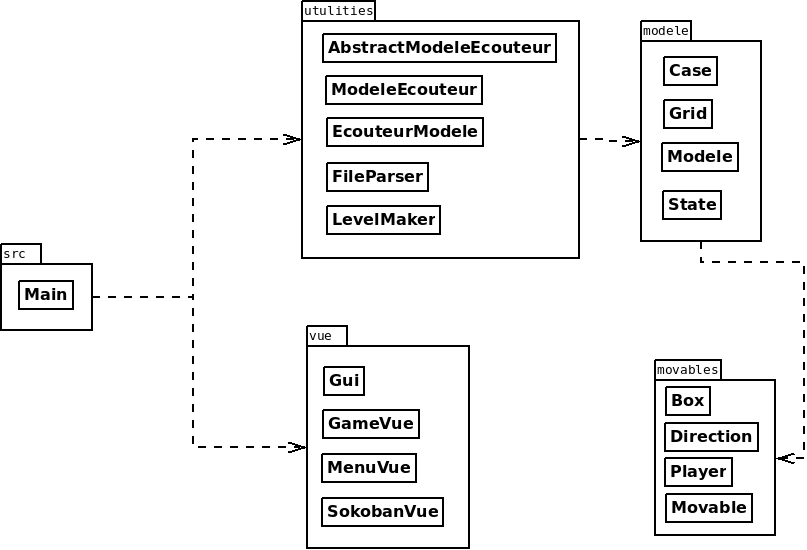
\includegraphics[scale=0.5]{Diagramme1.png}
\caption{Packages réalisés}
\end{figure}\\
Comme on le voit sur la figure l'application principale dépend de deux packages : vue et utulities qui dépend de modele, qui dépend lui même de movables.\\
Le diagramme ci-dessous représente le package modele, il contient les classes permettant le fonctionnement du jeu sans interface graphique.\\
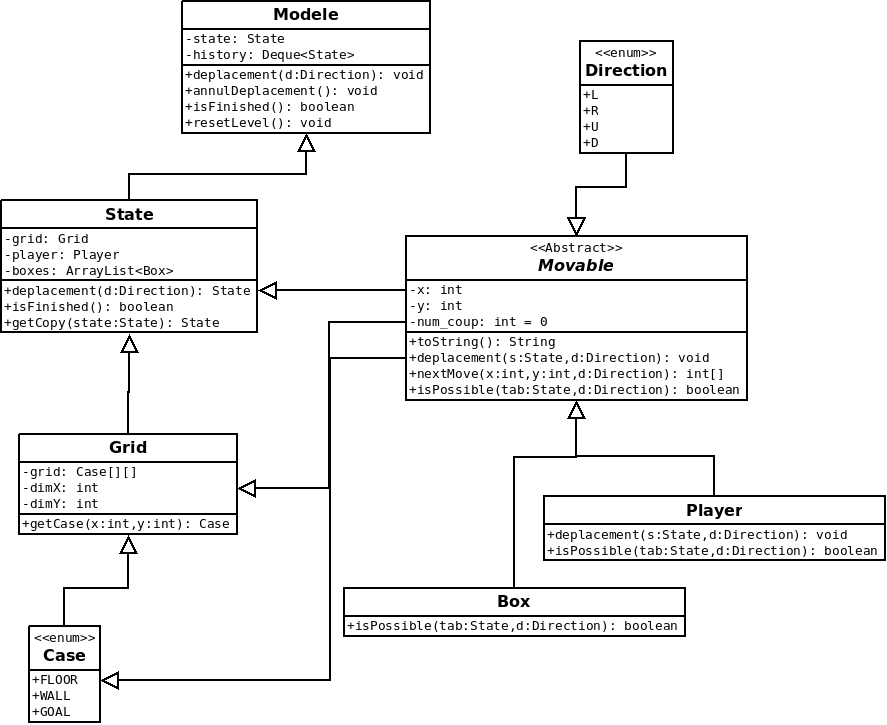
\includegraphics[scale=0.5]{Diagramme3.png}\\
Le diagramme ci-dessous représente le package vue, il contient les classes permettant l'affichage du jeu et le menu.\\
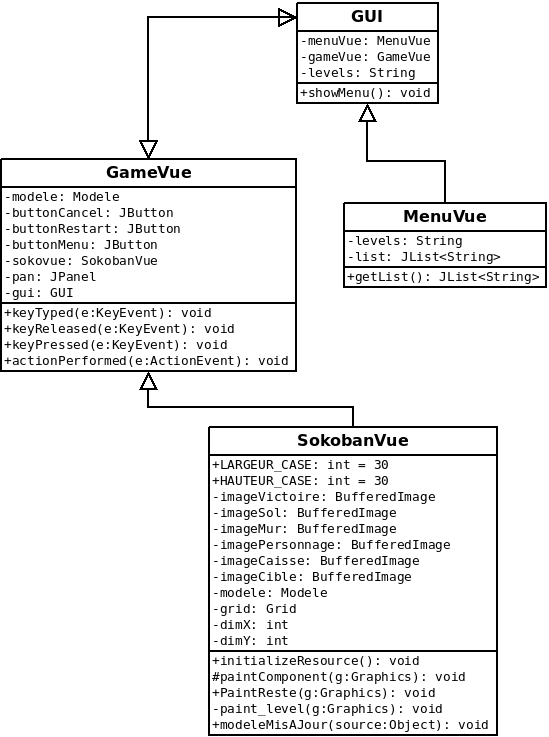
\includegraphics[scale=0.5]{Diagramme4.png}\\
\subsection{Cas d'utilisation}
Dans la partie suivante je vais vous présenter différents diagrammes de cas d'utilisation de notre Sokoban, mais  qu'est ce qu'un diagramme de cas d'utilisation, et bien c'est un moyen simple d'exprimer les besoins de notre jeu, il nous permet ainsi de recenser les différentes idées, qui seront par la suite implémenté à notre jeu.\\
\\
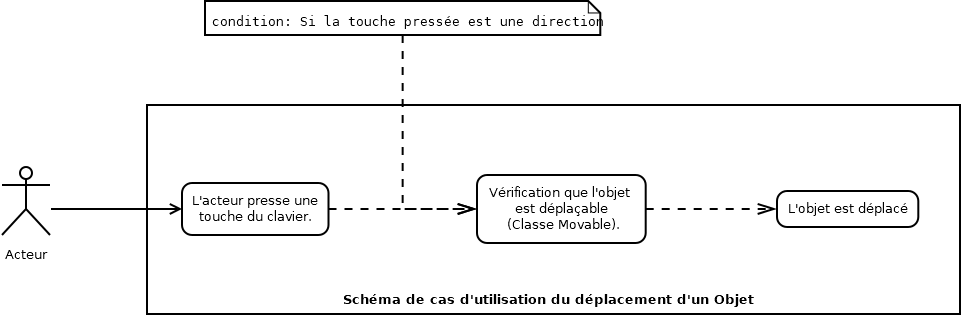
\includegraphics[scale=0.5]{Diagramme5.png}\\
Le diagramme ci-dessus correspond au différent évènement possible dans le cas où le joueur presserait une touche pour déplacer son personnage, on voit en effet que si le joueur presse une touche qui ne correspond pas au direction, le jeu ne fait rien, et que lorsque une touche de déplacement est pressée, on vérifie si l'objet que l'on souhaite déplacer est "movable".\\
\\
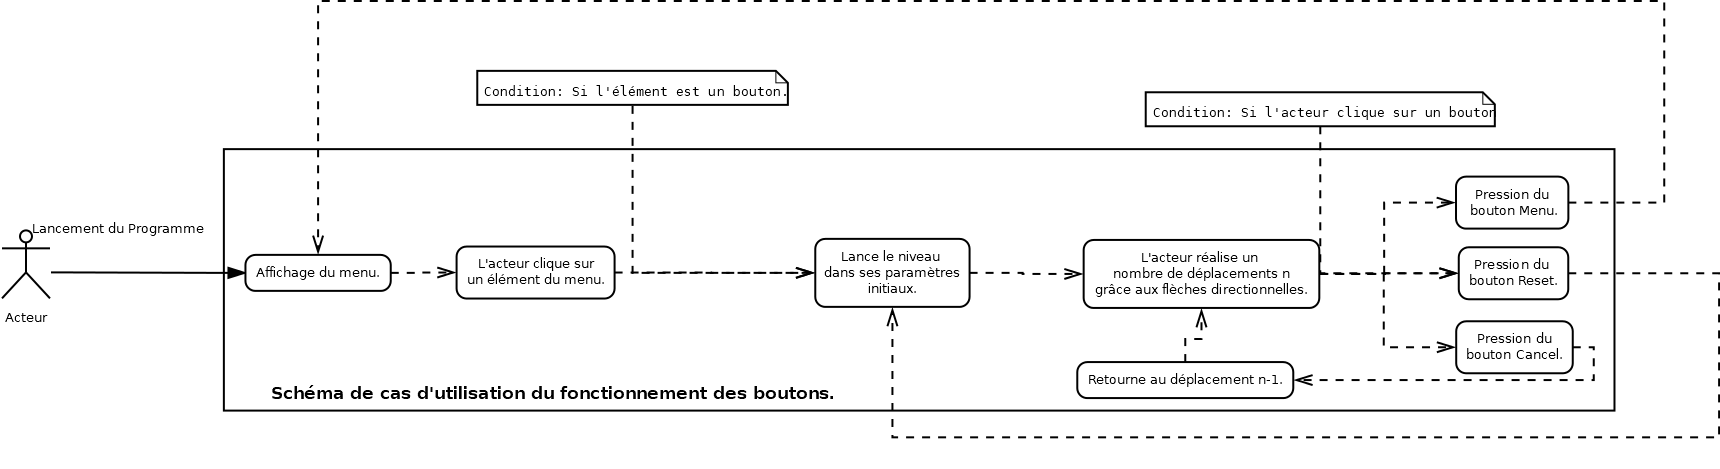
\includegraphics[scale=0.3]{Test.png}\\
Le diagramme ci-dessus correspond aux différentes actions réalisé lorsque le joueur clique sur un bouton, on voit que lorsque le joueur clique sur les boutons de niveau le jeu exécute alors le niveau sélectionné. Si un niveau est lancé on voit que le joueur possédant alors 3 boutons différent, un bouton "Menu" qui renvoie le joueur au menu de sélection des niveaux, un bouton "Reset" qui relance le niveau dans ses paramètres initiaux et un bouton "Cancel" qui renvoie le joueur un coup en arrière.

\section{Expérimentations et usages}

\subsection{Capture d'écrans}

Dans cette partie nous allons nous concentrer sur diverses expérimentations de notre jeu, afin de vérifier si nos méthodes fonctionnent comme il se doit. Pour commencer, nous avons tester la fonction 'deplacement' sur le premier niveau pour vérifier si le personnage se déplace correctement sur la grille lorsqu'on l'appelle.

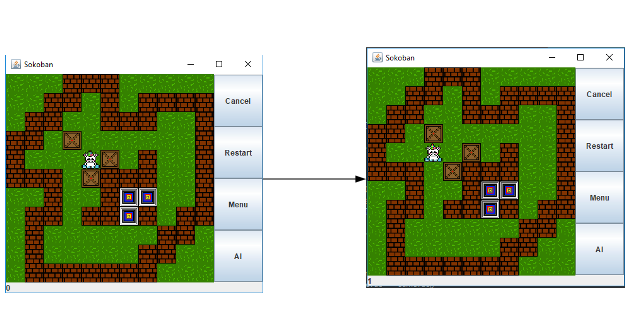
\includegraphics[scale=1]{Test1.PNG}\\

Sur la première capture d'écran, on peut voir l'état du jeu au stade initial avec notre personnage plaçé à un endroit précis. En utilisant la méthode 'deplacement' avec comme direction la gauche, notre personnage se déplace d'une case vers la gauche et l'on obtient comme résultat ce qui apparaît sur la deuxième capture d'écran. On remarque donc que le test de cette fonction est efficace car il y a bien eu la mise à jour du déplacement entre ces deux images.\\

Parallèlement, nous avons décidé de tester cette fonction sur le deuxième niveau en prenant la direction du haut, cependant un mur se trouve sur le chemin et l'on souhaite vérifier que le personnage ne puisse pas se déplacer dans ce cas là.

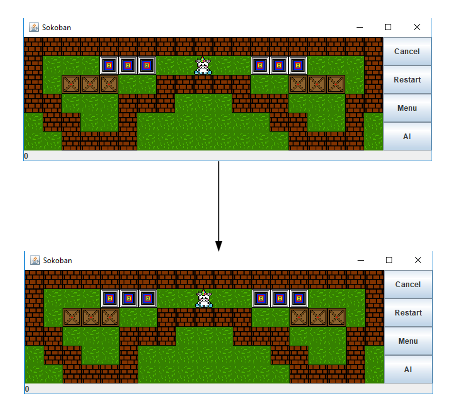
\includegraphics[scale=1.3]{Test2.PNG}\\

Sur la première capture d'écran, on peut voir l'état du jeu au stade initial avec notre personnage plaçé à un endroit précis. En utilisant la méthode 'deplacement' avec comme direction le haut, notre personnage devrait se déplacer d'une case vers le haut mais comme un obstacle est présent, le déplacement n'est donc pas effectué et le personnage ne se déplace pas, on peut le voir sur la deuxième capture d'écran. On remarque donc que le test de cette fonction est efficace car le personnage n'a pas bougé entre les deux images à cause du mur.\\

Dans un second temps, nous avons souhaité tester les boutons que nous avons implémentés à notre jeu, savoir s'ils réalisaient les actions demandés. Tout d'abord, nous avons vérifié l'efficacité du bouton 'Cancel' qui est censé reprendre le dernier coup joué et l'annuler.

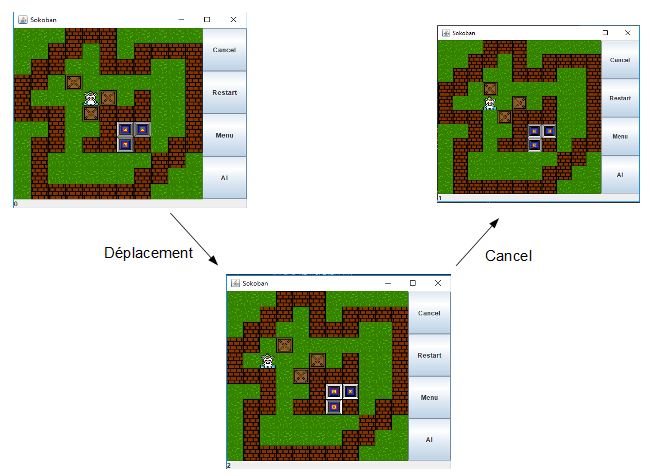
\includegraphics[scale=0.9]{Test3.PNG}\\

Sur la première image on peut observer le jeu à son état initial, on voit ensuite sur la deuxième image que le jour s'est déplacé deux fois vers la gauche. Le but de notre bouton 'Cancel' étant de retourner un coup en arrière, la troisième image présente l'efficacité de ce bouton car on voit bien que notre personnage est retourné sur la case précédent le dernier déplacement, c'est-à-dire qu'il est revenu une fois vers la droite.\\

Enfin, nous avons testé l'efficacité du bouton 'Restart' dont le but était de réinitialiser le niveau, c'est-à-dire, de reprendre le 'State' initial pour recommencer le niveau, au cas où l'on serait totalement bloqué et que le retour en arrière ne serait pas suffisant.

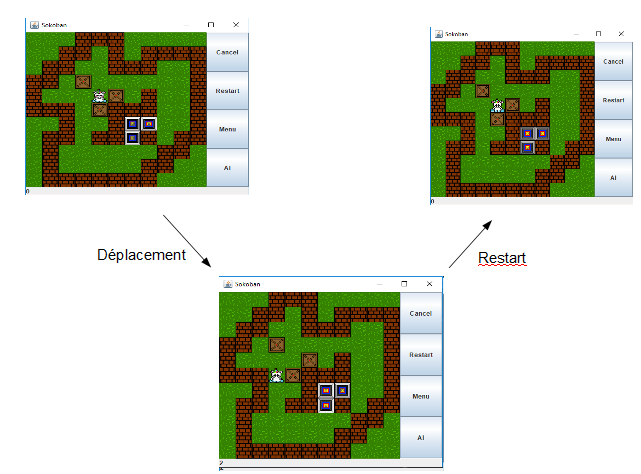
\includegraphics[scale=0.9]{Test4.PNG}\\

Sur la première image on peut voir le personnage à son emplacement initial comme précédemment, puis de la même manière le personnage se déplace d'une case vers la gauche puis d'une autre vers le bas. Cette fois-ci, notre but était de tester le bouton 'Restart' qui permettait de recommencer le niveau. C'est sur la troisième image que l'on remarque que le niveau est revenu à son état initial et donc que l'efficacité de notre bouton est vérifiée.\\ 

\subsection{Mesures de performance}

Afin de tester l'efficacité de la rapidité de notre programme nous avons alors décidé de lui implémenter une méthode permettant de mesurer ses performances, on calcule donc le temps pris par le programme pour générer le menu entre le moment où l'on demande à l'ordinateur d'exécuter le programme et le moment où le menu de notre jeu apparaît à l'écran, on constate alors que notre programme prend en moyenne 700 à 800ms pour réaliser cette opération.

En conclusion, ce temps nous montre que nous avons réussi à optimiser la vitesse d'évolution de notre programme.

\newpage

\section{Conclusion}

\subsection{Conclusion}

Pour conclure, ce projet fut éprouvant et compliqué, nous avons eu du mal à gérer notre temps entre l'apprentissage des différentes bibliothèques et la mise en place de tout ce que nous souhaitions réaliser. Cependant, nous avons fais du mieux que nous pouvions pour concevoir un jeu fonctionnel dans les temps avec une vue correcte et une tentative d'IA, certes peu fructueuse mais fait avec les moyens du bord.

Ce projet nous a malgré tout beaucoup apporté, en somme une meilleure approche du langage de programmation Java et du modèle M-VC vu en cours de POO. Mais aussi, nous avons pu profiter de ce projet pour affiner notre esprit d'équipe et notre organisation.

Nous sommes tout de même fier de notre travail même si nous avions beaucoup plus d'ambition à la base, cela reste un jeu agréable à parcourir.

\subsection{Améliorations possibles}

Toutefois, il reste de nombreux points qui pourraient être améliorés avec le temps, nous allons vous en présenter certains ici :

\begin{itemize}
\item L'ajout d'une nouvelle intelligence artificielle plus performante qui peut être interrompue à tout moment pour laisser place au joueur;
\item L'ajout de nombreux nouveaux niveaux afin d'accroître la durée de vie du jeu;
\item L'ajout d'un éditeur de niveaux qui permettra aux joueurs les plus talentueux de construire leurs propres niveaux;
\item L'ajout d'un mode deux joueurs coopératif afin de parcourir le jeu à plusieurs, une aide non négligable pour finir les niveaux les plus ardus;
\item Mise en place d'un chronomètre visible à l'écran , qui permettra au joueur de visualiser le temps pris à réaliser un niveau;
\item L'ajout d'un mode DualScreen (Ordinateur vs Humain) qui permettra de réaliser de nombreuses courses haletantes, Homme ou Machine, seul le plus rapide en sortira vainqueur.
\end{itemize}

\newpage

\section{Références}

\begin{thebibliography}{9}
\bibitem{1} Openclassrooms, Disponible sur \url{https://openclassrooms.fr}
\bibitem{2} Developpez.coms, Disponible sur \url{https://www.developpez.net/forum/}
\bibitem{3} Stackoverflow, Disponible sur \url{https://www.stackoverflow.com}
\bibitem{4} Wikipedia Sokoban, Disponible sur \url{ https://en.wikipedia.org/wiki/Sokoban}
\bibitem{5} Wikipedia Swing, Disponible sur \url{ https://en.wikipedia.org/wiki/Swing_(Java)}
\bibitem{6} Wikipedia AWT, Disponible sur \url{ https://en.wikipedia.org/wiki/Abstract_Window_Toolkit}
\bibitem{7} Javacodegeeks, Disponible sur \url{https://www.javacodegeeks.com/}
\bibitem{8} API Java, Disponible sur \url{https://docs.oracle.com/javase/7/docs/api/}
\bibitem{9} Guide pour Git, Disponible sur \url{http://rogerdudler.github.io/git-guide/index.fr.html}
\bibitem{10} Piskel, Disponible sur \url{https://www.piskelapp.com/}

\end{thebibliography}

\end{document}
